\documentclass{standalone}
\usepackage{tikz}
\usetikzlibrary{patterns, positioning}
\usepackage[sfdefault]{ClearSans} %% option 'sfdefault' activates Clear Sans as the default text font
\usepackage[T1]{fontenc}

\begin{document}
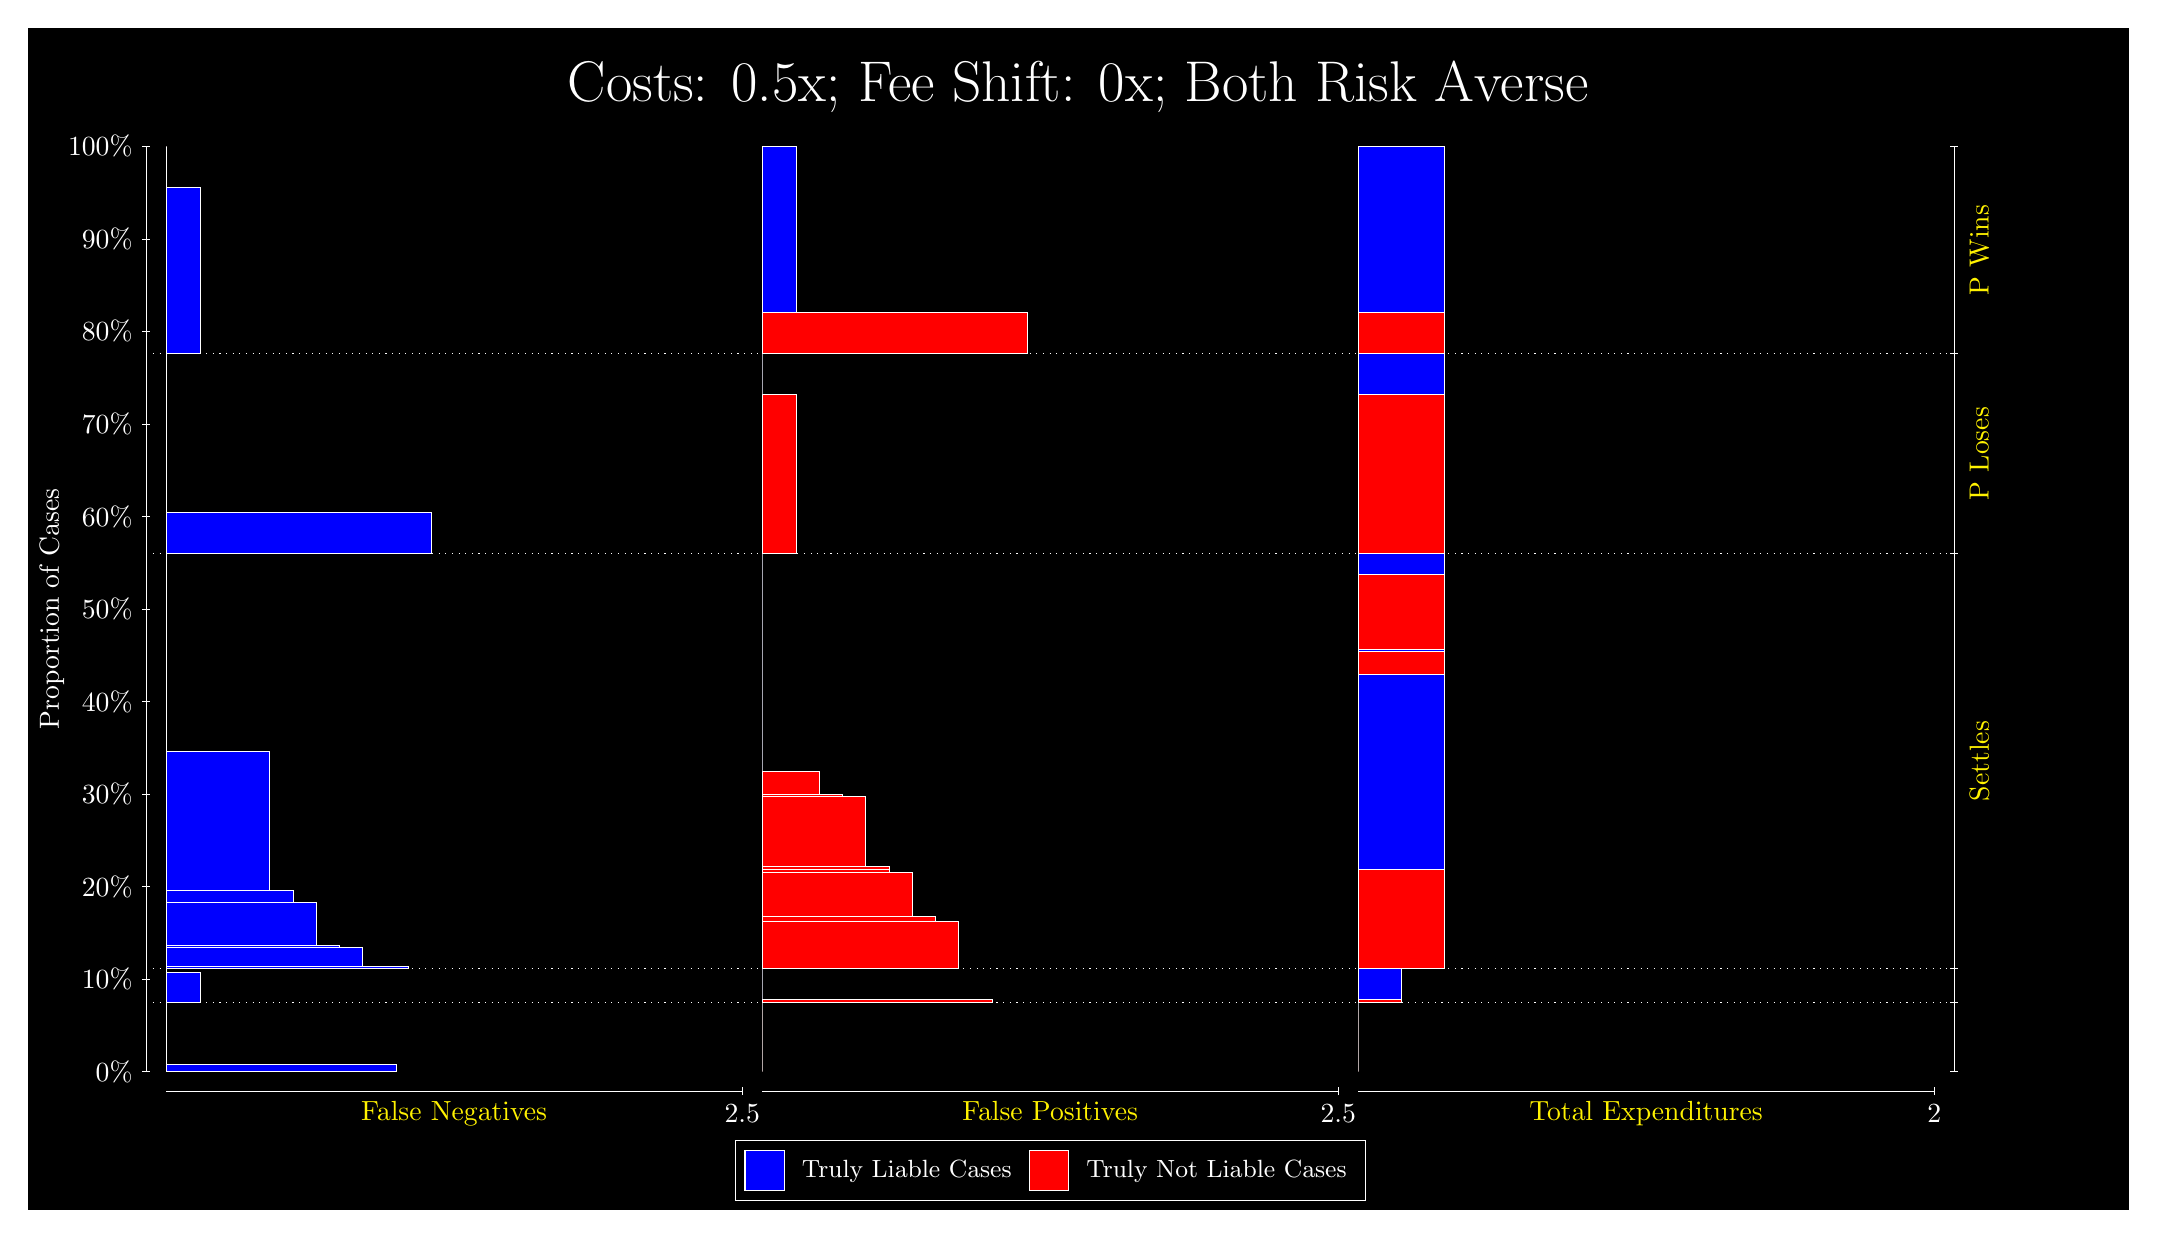
\begin{tikzpicture}
\draw[fill=black] (0,0) rectangle (26.667,15);
\draw[text=white] (0,13.5) rectangle (26.667,15) node[midway] {\huge Costs: 0.5x; Fee Shift: 0x; Both Risk Averse};
\draw[white, very thin] (1.5,1.75) -- (1.5,13.5);
\node[rotate=90, text=white, anchor=center] at (0.3, 7.625) {Proportion of Cases};
\draw[white, very thin] (1.45,1.75) -- (1.55,1.75);
\node[text=white, anchor=east] at (1.45, 1.75) {0\%};
\draw[white, very thin] (1.45,2.925) -- (1.55,2.925);
\node[text=white, anchor=east] at (1.45, 2.925) {10\%};
\draw[white, very thin] (1.45,4.1) -- (1.55,4.1);
\node[text=white, anchor=east] at (1.45, 4.1) {20\%};
\draw[white, very thin] (1.45,5.275) -- (1.55,5.275);
\node[text=white, anchor=east] at (1.45, 5.275) {30\%};
\draw[white, very thin] (1.45,6.45) -- (1.55,6.45);
\node[text=white, anchor=east] at (1.45, 6.45) {40\%};
\draw[white, very thin] (1.45,7.625) -- (1.55,7.625);
\node[text=white, anchor=east] at (1.45, 7.625) {50\%};
\draw[white, very thin] (1.45,8.8) -- (1.55,8.8);
\node[text=white, anchor=east] at (1.45, 8.8) {60\%};
\draw[white, very thin] (1.45,9.975) -- (1.55,9.975);
\node[text=white, anchor=east] at (1.45, 9.975) {70\%};
\draw[white, very thin] (1.45,11.15) -- (1.55,11.15);
\node[text=white, anchor=east] at (1.45, 11.15) {80\%};
\draw[white, very thin] (1.45,12.325) -- (1.55,12.325);
\node[text=white, anchor=east] at (1.45, 12.325) {90\%};
\draw[white, very thin] (1.45,13.5) -- (1.55,13.5);
\node[text=white, anchor=east] at (1.45, 13.5) {100\%};

\draw[white, very thin] (24.457,1.75) -- (24.457,13.5);
\draw[white, very thin] (24.407,1.75) -- (24.507,1.75);
\node[anchor=west] at (24.407, 1.75) {};
\draw[white, very thin] (24.407,2.6245) -- (24.507,2.6245);
\node[anchor=west] at (24.407, 2.6245) {};
\draw[white, very thin] (24.407,3.0586) -- (24.507,3.0586);
\node[anchor=west] at (24.407, 3.0586) {};
\draw[white, very thin] (24.407,8.3274) -- (24.507,8.3274);
\node[anchor=west] at (24.407, 8.3274) {};
\draw[white, very thin] (24.407,10.869) -- (24.507,10.869);
\node[anchor=west] at (24.407, 10.869) {};
\draw[white, very thin] (24.407,13.5) -- (24.507,13.5);
\node[anchor=west] at (24.407, 13.5) {};

\draw[white, very thin, fill=blue] (1.75,1.75) rectangle (4.6775,1.842);
\draw[white, very thin, fill=red] (1.75,1.842) rectangle (1.75,2.6245);
\draw[white, very thin, fill=blue] (1.75,2.6245) rectangle (2.1891,3.0142);
\draw[white, very thin, fill=red] (1.75,3.0142) rectangle (1.75,3.0586);
\draw[white, very thin, fill=blue] (1.75,3.0586) rectangle (4.8239,3.0824);
\draw[white, very thin, fill=blue] (1.75,3.0824) rectangle (4.5312,3.0862);
\draw[white, very thin, fill=blue] (1.75,3.0862) rectangle (4.2384,3.33);
\draw[white, very thin, fill=blue] (1.75,3.33) rectangle (3.9457,3.359);
\draw[white, very thin, fill=blue] (1.75,3.359) rectangle (3.6529,3.9009);
\draw[white, very thin, fill=blue] (1.75,3.9009) rectangle (3.3602,4.0465);
\draw[white, very thin, fill=blue] (1.75,4.0465) rectangle (3.0674,5.8218);
\draw[white, very thin, fill=red] (1.75,5.8218) rectangle (1.75,8.3274);
\draw[white, very thin, fill=blue] (1.75,8.3274) rectangle (5.1167,8.8482);
\draw[white, very thin, fill=red] (1.75,8.8482) rectangle (1.75,10.869);
\draw[white, very thin, fill=blue] (1.75,10.869) rectangle (2.1891,12.978);
\draw[white, very thin, fill=red] (1.75,12.978) rectangle (1.75,13.5);
\draw[white, very thin, fill=red] (9.3189,1.75) rectangle (9.3189,2.5325);
\draw[white, very thin, fill=blue] (9.3189,2.5325) rectangle (9.3189,2.6245);
\draw[white, very thin, fill=red] (9.3189,2.6245) rectangle (12.246,2.669);
\draw[white, very thin, fill=blue] (9.3189,2.669) rectangle (9.3189,3.0586);
\draw[white, very thin, fill=red] (9.3189,3.0586) rectangle (11.807,3.6519);
\draw[white, very thin, fill=red] (9.3189,3.6519) rectangle (11.515,3.7234);
\draw[white, very thin, fill=red] (9.3189,3.7234) rectangle (11.222,4.2793);
\draw[white, very thin, fill=red] (9.3189,4.2793) rectangle (10.929,4.3156);
\draw[white, very thin, fill=red] (9.3189,4.3156) rectangle (10.929,4.3558);
\draw[white, very thin, fill=red] (9.3189,4.3558) rectangle (10.636,5.2408);
\draw[white, very thin, fill=red] (9.3189,5.2408) rectangle (10.344,5.2763);
\draw[white, very thin, fill=red] (9.3189,5.2763) rectangle (10.051,5.5642);
\draw[white, very thin, fill=blue] (9.3189,5.5642) rectangle (9.3189,8.3274);
\draw[white, very thin, fill=red] (9.3189,8.3274) rectangle (9.758,10.348);
\draw[white, very thin, fill=blue] (9.3189,10.348) rectangle (9.3189,10.869);
\draw[white, very thin, fill=red] (9.3189,10.869) rectangle (12.686,11.391);
\draw[white, very thin, fill=blue] (9.3189,11.391) rectangle (9.758,13.5);
\draw[white, very thin, fill=red] (16.888,1.75) rectangle (16.888,2.5325);
\draw[white, very thin, fill=blue] (16.888,2.5325) rectangle (16.888,2.6245);
\draw[white, very thin, fill=red] (16.888,2.6245) rectangle (17.437,2.669);
\draw[white, very thin, fill=blue] (16.888,2.669) rectangle (17.437,3.0586);
\draw[white, very thin, fill=red] (16.888,3.0586) rectangle (17.986,4.3156);
\draw[white, very thin, fill=blue] (16.888,4.3156) rectangle (17.986,6.7949);
\draw[white, very thin, fill=red] (16.888,6.7949) rectangle (17.986,7.0828);
\draw[white, very thin, fill=blue] (16.888,7.0828) rectangle (17.986,7.1066);
\draw[white, very thin, fill=red] (16.888,7.1066) rectangle (17.986,8.0672);
\draw[white, very thin, fill=blue] (16.888,8.0672) rectangle (17.986,8.3274);
\draw[white, very thin, fill=red] (16.888,8.3274) rectangle (17.986,10.348);
\draw[white, very thin, fill=blue] (16.888,10.348) rectangle (17.986,10.869);
\draw[white, very thin, fill=red] (16.888,10.869) rectangle (17.986,11.391);
\draw[white, very thin, fill=blue] (16.888,11.391) rectangle (17.986,13.5);
\draw[white, dotted] (1.5,2.6245) -- (24.457,2.6245);
\draw[white, dotted] (1.5,3.0586) -- (24.457,3.0586);
\draw[white, dotted] (1.5,8.3274) -- (24.457,8.3274);
\draw[white, dotted] (1.5,10.869) -- (24.457,10.869);
\draw[white, very thin] (1.75,1.5) -- (9.0689,1.5);
\node[text=yellow, anchor=north] at (5.4094, 1.5) {False Negatives};
\draw[white, very thin] (9.0689,1.45) -- (9.0689,1.55);
\node[text=white, anchor=north] at (9.0689, 1.45) {2.5};

\draw[white, very thin] (9.3189,1.5) -- (16.638,1.5);
\node[text=yellow, anchor=north] at (12.978, 1.5) {False Positives};
\draw[white, very thin] (16.638,1.45) -- (16.638,1.55);
\node[text=white, anchor=north] at (16.638, 1.45) {2.5};

\draw[white, very thin] (16.888,1.5) -- (24.207,1.5);
\node[text=yellow, anchor=north] at (20.547, 1.5) {Total Expenditures};
\draw[white, very thin] (24.207,1.45) -- (24.207,1.55);
\node[text=white, anchor=north] at (24.207, 1.45) {2};



\node[text=yellow, centered, rotate=90] at (24.777, 5.693) {Settles};
\node[text=yellow, centered, rotate=90] at (24.777, 9.598) {P Loses};
\node[text=yellow, centered, rotate=90] at (24.777, 12.184) {P Wins};

\draw (12.978300999999998,1.5) node[draw=none] (baseCoordinate) {};
\begin{scope}[align=center]
        \matrix[scale=0.5, draw=white, below=0.5cm of baseCoordinate, nodes={draw}, column sep=0.1cm]{
            \node[rectangle, draw, minimum width=0.5cm, minimum height=0.5cm, fill=blue] {}; &
            \node[draw=none, font=\small, text=white] (B) {Truly Liable Cases}; &
            \node[rectangle, draw, minimum width=0.5cm, minimum height=0.5cm, fill=red] {}; &
            \node[draw=none, font=\small, text=white] (B) {Truly Not Liable Cases}; \\
            };
\end{scope}

\end{tikzpicture}
\end{document}